\documentclass{article}
\usepackage[utf8]{inputenc}
\usepackage[margin=0.5in,includefoot]{geometry}
\usepackage[export]{adjustbox}

% Header and Footer Setup
\usepackage{fancyhdr}
\pagestyle{fancy}
\fancyhead{}
\fancyfoot{}
\fancyfoot[R]{\thepage}
\renewcommand{\headrulewidth}{0pt}
\renewcommand{\footrulewidth}{0pt}
%
%Graphics Setup
\usepackage{graphicx}
\usepackage{float}
\usepackage{subfig}


%list setup
\usepackage{amssymb}
\renewcommand{\labelitemi}{$\blacktriangleright$}
\renewcommand{\labelitemii}{$\bullet$}
\renewcommand{\labelitemiii}{$\circ$}

%Source Code setup
\usepackage{xcolor}
\usepackage{listings}

\definecolor{mGreen}{rgb}{0,0.6,0}
\definecolor{mGray}{rgb}{0.5,0.5,0.5}
\definecolor{mPurple}{rgb}{0.58,0,0.82}
\definecolor{backgroundColour}{rgb}{0.95,0.95,0.92}

\lstdefinestyle{CStyle}{
    backgroundcolor=\color{backgroundColour},   
    commentstyle=\color{mGreen},
    keywordstyle=\color{magenta},
    numberstyle=\tiny\color{mGray},
    stringstyle=\color{mPurple},
    basicstyle=\footnotesize,
    breakatwhitespace=false,         
    breaklines=true,                 
    captionpos=b,                    
    keepspaces=true,                 
    numbers=left,                    
    numbersep=5pt,                  
    showspaces=false,                
    showstringspaces=false,
    showtabs=false,                  
    tabsize=2,
    language=C
}
%


\begin{document}

\begin{titlepage}

	\begin{flushright}
	\textsc{\large May 8, 2021} \\
	\end{flushright}
	\begin{center}
	\Large{\bfseries GTU Department of Computer Engineering \\ CSE344 - Spring 2021 \\ Homework 4 Report  } \\
	\end{center}
	\topskip0pt
	\vspace*{\fill}
	\begin{center}
	\Large{\bfseries Akif Kartal \\ 171044098 }
	\end{center}
	\vspace*{\fill}

\end{titlepage}

\cleardoublepage
\section{Problem Definition}
The problem is to implement \textbf{producer-consumer} problem by using POSIX threads and Semaphores as initiation to POSIX threads. 

\section{Solution}
The homework was finished as expected in homework pdf file. 
\subsection{Some Problems and Solutions}
\subsubsection{Semaphore Usage}
In order to provide synchronization between threads I used \textbf{6 POSIX unnamed semaphore} common between threads.
Followings are my semaphores;
\begin{lstlisting}[style=CStyle]
    sem_init(&run, 0, 0);
    sem_init(&mutex, 0, 1);
    sem_init(&empty, 0, 10);
    sem_init(&full, 0, 0);
    sem_init(&busy, 0, 0);
    sem_init(&dataMutex, 0, 1);
\end{lstlisting}
Usage purpose of each semaphore will be explained in detail coming pages.
\subsubsection{Thread Creation}
\subsubsection*{Main Thread}
Main thread is main function of program and it is responsible to initialize important variables such as queue, semaphores, money etc.
\subsubsection*{Thread G}
This thread is detached thread so its different than other. Also it is filling the queue therefore we need to \textbf{pass as parameter} the queue
to the this thread. Note that queue is \textbf{not} global it is in main thread. See the code;
\begin{lstlisting}[style=CStyle]
 pthread_attr_t attr;
 pthread_attr_init(&attr);
 pthread_attr_setdetachstate(&attr, PTHREAD_CREATE_DETACHED);

 /*create G thread*/
 queue *stdQueue = createQueue();
 pthread_create(&idG, &attr, threadG, (void *)stdQueue);
 pthread_attr_destroy(&attr);
\end{lstlisting}
\subsubsection*{Threads of student-for-hire}
Here, we have threads as many as number of student but important thing is \textbf{they will use same thread function}. Therefore, 
we need to design a communication mechanism between each student thread and main thread. My solution is following;
\subsubsection*{Setting Up the Student Threads}
Since, these threads are using same function somehow we need to distinguish each other. In order to do that we will pass an encapsulated data,
which contains information about student for each thread while creating. Note that after creating \textbf{they need to wait} until all of them
initialized with it's data. See the code;
\cleardoublepage
\begin{lstlisting}[style=CStyle]
 //data for each student to pass to the it's thread
 typedef struct info
 {
    char name[41];
    double price;
    double speed;
    double quality;
    double income;
    int solvedCount;
    int index;
    int isBusy;
    int isNotified;
    sem_t *notify;
    sem_t *startSolve;
    char currentHw;
    pthread_t id;
 } student;
\end{lstlisting}
In this data semaphores will be used to communicate and synchronize. Other variables are clear.
\subsubsection*{Creating Students}
\begin{lstlisting}[style=CStyle]
 //N = number of student(itu,ytu etc.)
 pthread_t tids[N];
 student hiredStds[N];
  
 /*create hired students threads and init them*/
 for (int i = 0; i < N; i++)
 {
    pthread_create(&tids[i], NULL, threadStd, &hiredStds[i]);
 }
 initStudents(hiredStds, fdStd, N, tids);
 mainPrintStudents(hiredStds,N);
 /*post that students can run now*/
 if (sem_post(&run) == -1)
        errExit("sem_post");
 /*student thread*/
 void *threadStd(void *info)
 {
    if (sem_wait(&run) == -1)
        errExit("sem_wait");
    if (sem_post(&run) == -1)
        errExit("sem_post");
    student *this = (student *)info;
    ...
 }
       
\end{lstlisting}

\subsubsection{Communication and Synchronization Problems}
\subsubsection*{Main Thread and Thread G}
I this two thread we have \textbf{producer-consumer} problem. In order to solve this problem I used 3 semaphore 
which are \textbf{full, empty, mutex}. \\ \\
Solution;
\cleardoublepage
\textbf{Producer(Thread G)}
\begin{lstlisting}[style=CStyle]
	do
    {
        nextHw = readOneChar(fdHw);
        if (nextHw != 'x' && !isFinished)
        {
            if (sem_wait(&empty) == -1)
                errExit("sem_wait");
            if (sem_wait(&mutex) == -1)
                errExit("sem_wait");
            if (isFinished)//money run out
                break;

            gNewHwMsg(nextHw,money);
            addRear(p, nextHw);

            if (sem_post(&mutex) == -1)
                errExit("sem_post");
            if (sem_post(&full) == -1)
                errExit("sem_post");
        }

    } while (nextHw != 'x' && !isFinished);
\end{lstlisting}
\textbf{Consumer(Main Thread)}
\begin{lstlisting}[style=CStyle]
	while (money > 0 && !isFinished)
	{
        if (sem_wait(&full) == -1)
            errExit("sem_wait");
        if (sem_wait(&mutex) == -1)
            errExit("sem_wait");
        if (!isQueueEmpty(stdQueue)){
            index = findStudent(hiredStds, getFront(stdQueue));
            if (hiredStds[index].price <= money)
            {
                if (sem_wait(&dataMutex) == -1)
                    errExit("sem_wait");
                    
                //remove hwk and update values  
                hiredStds[index].currentHw = removeFront(stdQueue);
                hiredStds[index].isNotified += 1;
                money = money - hiredStds[index].price;
                hiredStds[index].income += hiredStds[index].price;
                hiredStds[index].solvedCount += 1;
                
                //notify the selected student to start solving it
                if (sem_post(hiredStds[index].notify) == -1)
                    errExit("sem_post");
                if (sem_post(&dataMutex) == -1)
                    errExit("sem_post");
                    
                //wait first student to start
                if (sem_wait(hiredStds[index].startSolve) == -1)
                    errExit("sem_wait");

								if (sem_post(&mutex) == -1)
									errExit("sem_post");
								if (sem_post(&empty) == -1)
									errExit("sem_post");

            }
            else{
            	break;
        	}
        else{
            break;
        }
	}
\end{lstlisting}
In this code piece some semaphores belongs to main thread and hired student communication and synchronization.
Also, I determine Queue data structure \textbf{upper-bound limit is 10}.
\subsubsection*{Main Thread and Hired Students}
I this two thread we have \textbf{communication and synchronization} problems. In order to solve this problems I used 3 semaphores 
which are \textbf{run, busy, dataMutex}.Also in info for each student we are using \textbf{notify and startSolve} seamphores. \\ \\
Usage;
\begin{itemize}
	\item run: When a student thread created, it will wait to initialize its data by main thread.
	\item busy: When all students are busy main thread will wait until one student post to busy thread.
	\item dataMutex: Both students and main thread are updating student info, therefore in order to avoid race
	condition we will use this semaphore.
	\item notify: notify a student when it was chosen.
	\item startSolve: After notification was send wait the student to start \textbf{not} completely finished solving.
\end{itemize}
The solution of these problems is following;\\ \\
\textbf{Main Thread}
\begin{lstlisting}[style=CStyle]
	index = findStudent(hiredStds, getFront(stdQueue));
	if (index == -1)
	{
		//all of them are busy
		int counter;
		if (sem_getvalue(&busy, &counter) == -1)
			errExit("sem_get");
		if (counter > 0){
			if (sem_wait(&busy) == -1)
				errExit("sem_wait");
		}
		if (sem_wait(&busy) == -1)
			errExit("sem_wait");
		index = findStudent(hiredStds, getFront(stdQueue));
	}
	if (hiredStds[index].price <= money)
	{
		if (sem_wait(&dataMutex) == -1)
			errExit("sem_wait");
			
		//remove hwk and update values  
		hiredStds[index].currentHw = removeFront(stdQueue);
		hiredStds[index].isNotified += 1;
		money = money - hiredStds[index].price;
		hiredStds[index].income += hiredStds[index].price;
		hiredStds[index].solvedCount += 1;
		
		//notify the selected student to start solving it
		if (sem_post(hiredStds[index].notify) == -1)
			errExit("sem_post");
		if (sem_post(&dataMutex) == -1)
			errExit("sem_post");
			
		//wait first student to start
		if (sem_wait(hiredStds[index].startSolve) == -1)
			errExit("sem_wait");


	}
\end{lstlisting}
\cleardoublepage
\textbf{Hired Student}
\begin{lstlisting}[style=CStyle]
while (!isFinished || this->isNotified)
{
	stdWaitMsg(this->name);
	//wait notificition
	if (sem_wait(this->notify) == -1)
		errExit("sem_wait");
		
	if (this->isNotified){
		if (sem_wait(&dataMutex) == -1)
			errExit("sem_wait");
		this->isBusy = 1;
		stdSolvingMsg(this->name,this->price,money,this->currentHw);
		
		//release start mutex
		if (sem_post(this->startSolve) == -1)
			errExit("sem_post");
		if (sem_post(&dataMutex) == -1)
			errExit("sem_post");

		//simulate solving
		sleep(6 - (int)this->speed);

		if (sem_wait(&dataMutex) == -1)
			errExit("sem_wait");
			
		this->isNotified -= 1;
		this->isBusy = 0;

		if (sem_post(&dataMutex) == -1)
			errExit("sem_post");
		int counter;
		if (sem_getvalue(&busy, &counter) == -1)
			errExit("sem_get");
		if (counter == 0){
			if (sem_post(&busy) == -1)
				errExit("sem_post");
		}
	}
	else
		break;
}
\end{lstlisting}

In this solution 3 \textbf{binary} semaphore was used. These are \textbf{vac, cit, run}. \\ \\
\textbf{Note:} In this solution by using semaphores, I provided print message on screen
is happening like a queue. In other words, each citizen will print its message directly after getting an invite
from a vaccinator and vaccinator message. I had to do this otherwise messages on the screen will be messed up.
\subsubsection{Removing Resources and Exiting}
In order to run a cleaner method after finish, I used a cleaner method like this;
\begin{lstlisting}[style=CStyle]
    void removeAll()
    {
        if (sem_close(sem_full1) == -1)
            errExit("sem_close");
        if (sem_close(sem_empty) == -1)
            errExit("sem_close");
        if (sem_close(sem_full2) == -1)
            errExit("sem_close");
        if (sem_close(sem_run) == -1)
            errExit("sem_close");
        if (sem_close(sem_mutex) == -1)
            errExit("sem_close");
        if (sem_close(sem_vac) == -1)
            errExit("sem_close");
        if (sem_close(sem_cit) == -1)
            errExit("sem_close");
        sem_unlink("mutex344");
        sem_unlink("full344");
        sem_unlink("empty344");
        sem_unlink("full3442");
        sem_unlink("whorunfirst");
        sem_unlink("wait_vaccinator");
        sem_unlink("wait_citizen");
        shm_unlink(memoryName); //generic data
        shm_unlink(helperMemory); //current cit pid
    }
    
\end{lstlisting}
\cleardoublepage
\textbf{Usage: }
\begin{lstlisting}[style=CStyle]
    void cleanAndExit()
    {
        
        if (processInfo.type == PARENT)
        {
            reapDeadChildren();
            if (close(biontech->fd) < 0)
            {
                errExit("close file error!");
            }
        }
        else
        {
            removeAll();
        }
        exit(EXIT_SUCCESS);
    }
    
\end{lstlisting}
\subsubsection{Reaping Dead Children}
In order not to let zombie process, I used waitpid to wait dead children. Example;
\begin{lstlisting}[style=CStyle]
    void reapDeadChildren()
    {
        pid_t childPid;
        int status;
        while ((childPid = waitpid(-1, &status, 0)) > 0);
        if (childPid == -1 && errno != ECHILD)
            errExit("waitpid");
    }
\end{lstlisting}
\subsubsection{CTRL-C Handling}
In order to give a message on CTRL-C interrupt, I used \textbf{sigaction} function from \textbf{signal.h} library.
Also, in midterm pdf there is no force to print a message on CTRL-C interrup, therefore I didn't give any message.
\begin{lstlisting}[style=CStyle]
    //handler function
    void exitHandler(int signal)
    {
        if (signal == SIGINT)
        {
            int savedErrno = errno;
            cleanAndExit();
            errno = savedErrno;
        }
    }
\end{lstlisting}
There is no message, give resources back and exit elegantly.
\section{References that was used} 
While doing this howemork following references was used;
\begin{itemize}
	\item Course Textbook Listing 26-5: Reaping dead children via a handler for SIGCHLD
	\item Week-8 slides synchronization: Bounded buffer case in producer consumer problem.
\end{itemize}
\cleardoublepage
\section{Test Result}
I tried to obey output example in midterm pdf. In following output all decisions belongs to CPU. \\ \\
A simple test result is following;
\begin{figure}[H]
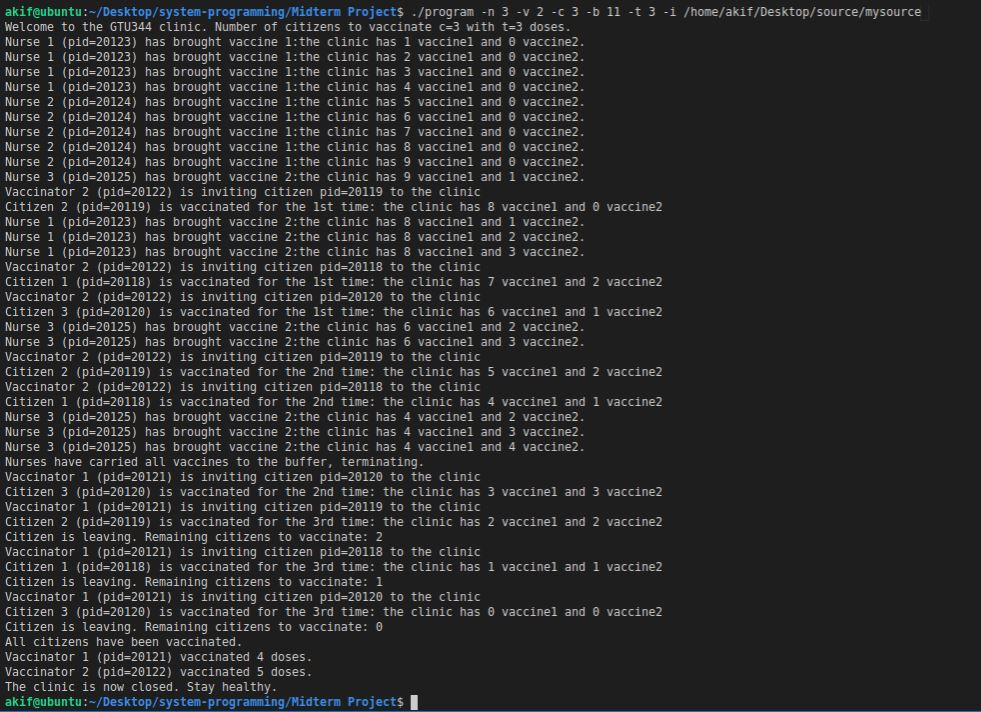
\includegraphics[width=1\textwidth, left]{result.JPG}
\caption[Optional caption]{}
\label{}
		
\end{figure}                              

\end{document}